\documentclass[a4paper,12pt]{article}
\usepackage[osf]{mathpazo}
\usepackage{ms}
\usepackage{natbib}
\usepackage{lineno}
\usepackage{graphicx}
\usepackage{caption}
\modulolinenumbers[5]
\linenumbers

\pdfminorversion=3

\makeatletter
\renewcommand{\@biblabel}[1]{\quad#1.}
\makeatother

% Disable words breaking over lines for final submission:
\raggedright

% Abbreviate "Figure" to "Fig." in captions:
\renewcommand{\figurename}{Fig.}

\title{How much of the world is woody?}
\author{
Richard G. FitzJohn$^{\dag, 1, 2}$, Matthew W. Pennell$^{\dag,3,4, *}$, Amy E. Zanne$^{5,6}$,\\ Peter F. Stevens$^{7,8}$, David C. Tank$^{3}$, and William K. Cornwell$^{9, 10}$
}
\date{}
\affiliation{\noindent{\footnotesize
$^\dag$ These authors contributed equally\\
$^1$ Biodiversity Research Centre and Department of Zoology,
University of British Columbia, Vancouver, BC V6G 1Z4, Canada\\
$^2$ Department of Biological Sciences, Macquarie University, Sydney, NSW 2109, Australia \\
$^3$ Department of Biological Sciences and Institute for Bioinformatics and Evolutionary Studies, University
of Idaho, Moscow, ID 83844, U.S.A.\\
$^4$ National Evolutionary Synthesis Center, Durham, NC 27705, U.S.A.\\
$^5$ Department of Biological Sciences, George Washington University,
Washington, D.C. 20052, U.S.A.\\
$^6$ Center for Conservation and Sustainable Development, Missouri Botanical Garden, St. Louis, MO, 63121, USA \\
$^7$ Department of Biology, University of Missouri, St. Louis, MO
63166, U.S.A.\\
$^8$ Missouri Botanical Garden, PO Box 299, St Louis, MO 63166-0299\\
$^{9}$ Department of Systems Ecology, VU University, 1081 HV
Amsterdam, The Netherlands\\
$^{10}$ Evolution \& Ecology Research Centre, School of Biological, Earth and Environmental Sciences, University of New South Wales, Sydney 2052 NSW, Australia\\
$^*$ Correspondence author. Email: \texttt{mwpennell@gmail.com}}\\

\vfill
% \raggedright, no line numbers, \pagestyle{empty}, copy and paste,
% remove figures (draft mode would be faster) and don't count
% supplement.
% \paragraph{Word-count:} 4179 words
%\paragraph{Manuscript elements:} Fig.~1-3 (bw in print), Appendix.
%\paragraph{Article type:} Note.
}
\mstype{Future Directions paper}
\runninghead{How much of the world is woody?}
\keywords{Databases, Determinantes of plant community diversity and structure, Functional diversity, Herbaceousness, Macroecology, Sampling bias, Woodiness}

\begin{document}
% \raggedright
% \pagestyle{empty}

\mstitlepage
\parindent=1.5em
\addtolength{\parskip}{.3em}

\begin{abstract}
\singlespacing
\begin{enumerate}
\item The question posed by the title of this paper is a basic one,
  and it is surprising that the answer is not known. Recently
  assembled trait datasets provide an opportunity to address this, but
  scaling these datasets to the global scale is challenging because of
  sampling bias.  Although we currently know the growth form of tens
  of thousands of species, these data are not a random sample of
  global diversity; some clades are exhaustively characterised, while
  others we know little--to--nothing about.
  % 
\item Starting with a database of woodiness for 39,313 species of
  vascular plants (12\% of taxonomically resolved species, 59\% of
  which were woody), we estimated the status of the remaining
  taxonomically resolved species by randomisation.  To compare the
  results of our method to conventional wisdom, we informally surveyed
  a broad community of biologists.  No consensus answer to the
  question existed, with estimates ranging from 1\% to 90\% (mean:
  31.7\%).
  % #rstats
  % nrow(load.woodiness()) # 39313
  % sum(dat.g$K) / sum(dat.g$N) # 0.12 -- fraction known
  % sum(dat.g$W) / sum(dat.g$K) # 0.59 -- fraction woody
  % d.survey <- load.survey()
  % range(d.survey$Estimate) # 1 - 90
  % mean(d.survey$Estimate)  # 31.7
\item After accounting for sampling bias, we estimated the proportion
  of woodiness among the world's vascular plants to be between 45\%
  and 48\%.  This was much lower than a simple mean of our dataset and
  much higher than the conventional wisdom.
  % #rstats
  % round(100*range(c(res.b$overall.p, res.h$overall.p)))
  % round(100*res.b$overall.p, 1) # 45.6 (45.3 -- 45.9)
  % round(100*res.h$overall.p, 1) # 47.6 (47.0 -- 48.2)
\item \emph{Synthesis}: Alongside an understanding of global taxonomic
  diversity (i.e., number of species globally), building a functional
  understanding of global diversity is an important emerging research
  direction.  This approach represents a novel way to account for
  sampling bias in functional trait datasets and to answer basic
  questions about functional diversity at a global scale.
\end{enumerate}
\end{abstract}

\newpage
\doublespacing
\section{Introduction}

The distinction between a woody and non--woody growth--form is
probably the most profound contrast among terrestrial plants and
ecosystems: for instance, a forest is dominated by woody taxa 
while a grassland is dominated by herbs.  The recognition of the fundamental
importance of this divide dates back at least to \textit{Enquiry into
  Plants} by Theophrastus of Eresus (371--287 BC), a student of
Plato and Aristotle, who began his investigation into plant form and
function by classifying the hundreds of plants in his garden into
woody and herbaceous categories \citep{theophrastus1916enquiry}.

The last two thousand years of research into wood since Theophrastus
classified his garden have uncovered its origin in the early Devonian
($\sim$400 Mya; \citealt{gerrienne2011simple}); that prevalence of
woodiness varies with climate \citep{Molesheihgt}; that wood has been
lost many times in diverse groups, both extant and extinct
\citep{judd1994}, often as an adaptation to freezing temperatures
\citep{Zanne}; that it has also been gained many times,
particularly on island systems \citep{Carlquist1974,Givnish1998};
and that many different forms of pseudo--woody growth
habit have appeared across groups that have lost true woodiness or
diverged before true woodiness evolved \citep{Cornwellwood}.  We know
about its mechanical properties and developmental pathways, its
patterns of decomposition and their effects on ecosystem function
\citep{Cornwellwood}, and that woody and herbaceous species have
markedly different rates of molecular evolution \citep{SmithDonoghue}.
%
However, we have no idea about what proportion of species in the world
are actually woody.

Recently assembled functional trait datasets provide an opportunity to
address this question. However, such datasets are, almost without
exception, biased samples of global diversity.  Researchers collect
data for specific questions on a local scale, and assembling these
local datasets creates a useful resource \citep{kattge2011try}.  But
as with GenBank's assembly of genetic data
\citep{smith2011understanding}, the simple compilation of data is not
an unbiased sample, and these initial sampling biases will, in turn,
bias downstream analyses.  Understanding and accounting for the biases
in these datasets is an important and necessary next step.

We sought to develop an approach that accounts for this bias.  In
doing so, we were able to re--ask Theophrastus' 2000--year old
question at a global scale: how many of the world's plant species are
woody?
%
We also sought to understand how well scientists were able to overcome
this bias and make a reasonable estimate.  To do this, we took the
unconventional approach of coupling our analysis with an informal
survey in which we asked our question to the broader community of
botanists and other biologists.

\section{Materials and Methods}

\subsection{Dataset}

We used a recently assembled database with growth--form data for
49,061 vascular plant species (i.e., lycopods, ferns, gymnosperms and
angiosperms), which is the largest such database assembled to date
\citep[][available on the Dryad data repository; doi:10.5061/dryad.63q27/2]{Zanne}.
%
This database uses a functional definition of woodiness: woody species
have a prominent above--ground stem that persists through time and changing
environmental conditions and herbaceous species lack such a stem --- 
a definition originally suggested by Asa Gray \citeyearpar{gray1887elements}. 
\citet{Zanne}
chose this simple definition because it best characterised the functional
aspect of growth form that they investigated, allowing them to compare 
species that maintain an above--ground stem through freezing conditions to 
ephemeral species that avoid freezing conditions.  More precise definitions 
that rely on lignin content and/or secondary vascular tissue from a bifacial
cambium are problematic because there are many exceptions depending on tissue 
type, times of development, or environmental conditions 
\citep{Groover2005, Spicer2010, Rowe2012}.  
Because our analyses and survey were based on this database, 
we present this functional definition of woodiness here for clarity 
(see \citet{Zanne} for a discussion of the various definitions of woodiness, 
their merits, and pitfalls).  Note that in addition to species producing
secondary xylem, this definition
classifies, among other groups, palms, tree ferns and bamboo as
woody.

As with all large data assemblies, the underlying datasets were collected 
for a variety of research goals. For example, a number of the datasets come
from forestry inventories, which, of course, are biased towards recording
woody species. Other sources of sampling bias, including geographically restricted sampling 
in many sub-datasets, may be less obvious but
nonetheless may have major implications for the inferences drawn from 
aggregate databases.

Because the effort to organise plant taxonomy, especially synonymy, is
on--going, there was uncertainty regarding the status of many plant
names.
%
To bring species binomials to a common taxonomy among datasets, names
were matched against accepted names in the Plant List
\citep{ThePlantList}.  Any binomials not found in this list were
matched against the International Plant Name Index
(http://www.ipni.org/) and Tropicos (http://www.tropicos.org/).
Potential synonymy in binomials arising from the three lists was
investigated using the Plant List tools \citep{ThePlantList}.  
% NOTE: This is the cleaning step done by `load.woodiness()`.
As a result of this cleaning, the number of species in the final
dataset was reduced from 49,061 to 39,313.
% #rstats
% nrow(read.csv("data/zae/GlobalWoodinessDatabase.csv")) # 49061
% nrow(load.woodiness())                                 # 39313

Theophrastus recognised both the fundamental importance of the
distinction between woody and herbaceous plants, and that this
distinction is in some cases difficult to make.  There are two ways
that species were recorded as ``variable'' in form
\citep{beaulieuHiddenRates}.  First, different records of a single
species may conflict in growth form (having both records of woodiness
and herbaceousness); this affected 307 of the 39,313 species in the
database.
% #rstats
% dat <- load.woodiness()
% tmp <- parse.count(dat$woodiness.count)
% multi <- rowSums(tmp > 0) > 1
% sum(multi)        # 307
% nrow(tmp)         # 39313
% mean(multi) * 100 # 0.8%
Second, 546 species (1.4\%) were coded as variable.
% #rstats
% sum(tmp[,"V"] > 0)  # 546
% nrow(tmp)           # 39313
% mean(tmp[,"V"] > 0) # 0.014
% sum(tmp[,"V"] > 0 & rowSums(tmp[,c("H", "W")]) > 0) # 53 (of 546)
Following \citet{beaulieuHiddenRates}, we coded species in these
groups as ``woody'' or ``herbaceous'' when a majority of records were
either ``woody'' or ``herbaceous'', respectively, and for these
species, records of ``variable'' do not contribute to the analysis.
%
%
Our final database for the main analysis contained 38,810 records with
both information on woodiness and documented taxonomy --- 15,957 herbs
and 22,853 woody species.  
% #rstats
% sum(dat.g$K) # 38810 -- known species
% sum(dat.g$H) # 15957 -- herbs
% sum(dat.g$W) # 22853 -- woody species
This included records from all flowering plant orders currently
accepted by APG III \citep{APG3} and the fern taxonomy of
\citet{apweb}, covering 15,232 genera and 465 families.
% #rstats
% sapply(dat.g[c("genus", "family")], function(x) length(unique(x)))
The 503 species excluded at this step had identical numbers of records
of being woody and herbaceous.
% #rstats
% nrow(dat) - sum(dat.g$K)    # 503
% sum(tmp[,"W"] == tmp[,"H"]) # 503
We also ran analyses where we coded growth forms by treating species
with \emph{any} record of woody or variable as ``woody'' (and
similarly for herbaceous), using all 39,313 species.  Neither of these
cases are likely to be biologically realistic but allowed us to
evaluate the maximal possible effect of mis--coding variable species.

\subsection{Estimating the percentage of species that are woody}

To estimate the percentage of species that are woody, we cannot simply
use the fraction of species within our trait database that are woody
(22,853 of 38,810 = 59\%) as these records represent a biased sample
of vascular plants.
% #rstats
% sum(dat.g$W) # 22853 -- woody
% sum(dat.g$K) # 38810 -- known
% sum(dat.g$W) / sum(dat.g$K) # 0.59 -- fraction
For example, most Orchidaceae are probably herbaceous; we have only
one record of woodiness among the 1,573 species for which we have
data.
% #rstats
% i.orc <- dat.g$family == "Orchidaceae"
% sum(dat.g$K[i.orc]) # 1573 -- known Orchidaceae
% sum(dat.g$W[i.orc]) # 1    -- woody Orchidaceae
However, the fraction of Orchidaceae species with known data (1,573 of
27,801 = 6\%)
% sum(dat.g$K[i.orc]) #  1573 -- known Orchidaceae
% sum(dat.g$N[i.orc]) # 27801 -- number of Orchidaceae
% sum(dat.g$K[i.orc]) / sum(dat.g$N[i.orc]) # 0.55 -- fraction known
is much lower than the overall rate of knowledge for all vascular
plants (38,810 of 284,732 = 12\%), which will upwardly bias the global
estimate of woodiness.
% #rstats
% sum(dat.g$K) #  38810 -- known vascular
% sum(dat.g$N) # 284732 -- total vascular
% sum(dat.g$K) / sum(dat.g$N) # 0.12 -- fraction known
Conversely, systematic under--sampling of tropical species would bias
the global woodiness estimate downwards, as tropical floras are
thought to harbour a greater proportion of woody species than
temperate ones \citep{Molesheihgt}.

We developed a simple method to account for this sampling bias when
estimating the percentage of woody species.  In our approach, we treat
each genus separately, and in all cases know that there are are $n_w$
woody and $n_h$ herbaceous species and a total of $N$ species in the genus.
%
For example, the genus \textit{Microcoelia} (Orchidaceae) has 30
species in total, and we know that 12 are herbaceous and none are
known to be woody ($N = 30$, $n_w = 0$, $n_h = 12$). We do not know
the state of the remaining 18 species, so the true number of woody
species, $N_w$, must lie between 0 and 18. In general, we cannot
assume that these species are all herbaceous, even though both
biological and mathematical intuition suggest that most of them will
be.
% #rstats
% i.mic <- which(dat.g$genus == "Microcoelia")
% dat.g[i.mic,c("N", "W", "H")]   # 30, 0, 12
% dat.g$N[i.mic] - dat.g$K[i.mic] # 18

We used two different approaches for imputing the values of these
unknown species. First, we assumed that the known species were sampled
without replacement from a pool of species with $N_w$ woody and $N_h$
herbaceous species ($N_w + N_h = N$), following a hypergeometric
distribution. The probability that $x$ of the species of unknown state
are woody ($x = 0, 1, \ldots, N - n_w - n_h$) is proportional to
\begin{equation}
  \Pr(N_w = x) \propto {n_w + x \choose n_w}
  {N - n_w - x \choose n_h}
\end{equation}
Under this sampling model, the more species for which we do not have data,
the greater the uncertainty in our estimates for the proportion of species
which are woody.
%
For \textit{Microcoelia} this model gives a 42\% probability that all
species are herbaceous, and a 90\% chance that at most 3 species
are woody.
% #rstats
% # Based on the code inside rhyper2()
% n <- dat.g$N[i.mic]; w <- dat.g$W[i.mic]; h <- dat.g$H[i.mic]
% xw <- seq(w, n - h) # possible number of woody species
% xh <- n - xw
% ph <- dhyper(h, xh, xw, h + w) # probability of (xh[i], xw[i])
% ph <- ph / sum(ph) # normalise
% ph[1]        # 0.42 -- all species herbaceous
% sum(ph[1:4]) # 0.90 -- at most 3 species woody
This approach probably overestimates the number of woody species in
this case, and in other cases where all known species are woody (e.g.,
\textit{Actinidia} [Ericaceae]) it will probably underestimate the
number of species that are woody. We see this as corresponding to a
weak prior on the shape of the distribution of the fraction of woody
species within a genus and will refer to this as the ``weak prior''
approach because it weakly constrains the state of missing species.

However, the distribution of woodiness among genera and families is
strongly bimodal; most genera are either all--woody or all--herbaceous
(Fig. \ref{fig:distribution-genera}, \ref{fig:distribution-family}, and 
\citealt{sinnott1915evolution}).  Among the 791 genera with at least 10
records, 411 are entirely woody, 271 are entirely herbaceous, and only
58 have between 10\% and 90\% woody species. Qualitatively similar patterns
hold at both the level of family and order, though the distribution
becomes progressively less bimodal as one moves up the taxonomic hierarchy 
(Figs. \ref{fig:distribution-family} and \ref{fig:distribution-order}). 
As a result, knowing the state of a handful of species within a genus 
can give a reasonable guess at the state of remaining species.
% #rstats
% tmp <- dat.g$p[dat.g$K >= 10] # select genera with 10 records
% length(tmp)              # 791 -- genera with at least 10 records
% sum(tmp == 1)            # 411 -- 100% woody
% sum(tmp == 0)            # 268 -- 100% herbaceous
% sum(tmp > 0 & tmp < 1)   # 106 -- variable
% sum(tmp > .1 & tmp < .9) #  58 -- interestingly variable

To model the other extreme of sampling, we used an approach where we
computed the observed fraction of woody species 
\[p_w = n_w / (n_w +n_h)\] 
and sampled the state of the unobserved species using a
binomial distribution, which represents the case of sampling
with replacement. In this case the probability that $x$ of the species
are woody is:
\begin{equation}
  \Pr(x = k) = {N - n_w - n_h \choose k - n_w} 
  p_w^k (1-p_w)^{N - n_h - k}.
\end{equation}
%
In cases where all known species are woody (or herbaceous as in
\textit{Microcoelia}) this will assign all unknown species to be woody
(or herbaceous). For such genera, increasing the number of unobserved
species will not increase the uncertainty in the estimate, in contrast
to the weak prior sampling approach.
%
We therefore see the binomial sampling approach as corresponding to a
very strong prior on the bimodal distribution of woodiness among
genera, and we will refer to this as the ``strong prior'' approach
because it more strongly constrains the state of missing species
within genera with no known polymorphism.  While neither of these
approaches is ``correct'', they probably span the extremes of possible
outcomes.
%
In polymorphic genera the two approaches will give similar results,
especially where the number of unknown species is relatively large.

For genera where there was no information on woodiness for any
species, we sampled a fraction of species that might be woody from
the empirical distribution of woodiness fractions \textit{among
  genera} within the same order. We did this after imputing the
missing species values within those other genera. So, if a genus is
found in an order with genera that had woodiness fractions of $\{0, 0,
0.1, 1\}$ we would have approximately a 50\% chance of sampling a 0\%
woodiness fraction for a genus, with probabilities from 0.1 to 1 being
fairly evenly spread.  Given this woodiness fraction, we then sampled
the number of species that are woody from a binomial distribution with
this fraction and the number of species in the genus as its
parameters.
% #rstats
% hist(quantile(c(0, 0, 0.1, 1), runif(10000)))

In addition to the number of species known to be woody and herbaceous,
we also require an estimate of the number of species per genus.  For this, we
used the number of accepted names within each genus in the Plant List
\citep{ThePlantList}. The taxonomic resources were compiled by \citet{Zanne}
are on available on Dryad (doi:10.5061/dryad.63q27/1). 

For each genus, we sampled the states of unobserved species, from
either the hypergeometric or binomial distribution, parametrised from
the observed data for that genus.
%
For each sample we can then combine these estimates to compute the
number (or fraction) of species that are woody at higher taxonomic
levels (family, order or vascular plants).  We repeated this sampling
1,000 times to generate distributions of the number (or fraction) of
species that are woody.
%
The R code and data to replicate this analysis are available on github
(\texttt{https://github.com/richfitz/wood}) and are included
as supplemental material.

\subsection{Survey}

In estimating the number of species within Angiosperm families,
\citet{joppa2010} found that expert opinion generally agreed closely
with estimates from a statistical model.  We were interested in
whether a consensus answer existed --- even if not formalised in the
literature --- and if so, whether it was consistent with our
estimates.
% 
We created an English-language survey (which we also translated into
Portuguese) asking for an estimate of the percentage of species that
are woody according to the above definition.  We also asked
respondents to indicate their level of familiarity with plants, level
of formal training, and the country in which they received their
training. We sent out the survey to several internet mailing lists and
social media websites (see Appendix for details on the
survey).

\section{Results}

Across all vascular plants, we estimated the fraction of woody species
to be between 45\% and 48\%.
% #rstats
% round(100*res.b$overall.p, 1) # 45.6 (45.3 -- 45.9)
% round(100*res.h$overall.p, 1) # 47.6 (47.0 -- 48.2)
Specifically, using our strong prior sampling approach (binomial
distribution) we estimated 45.6\% of species are woody (95\%
confidence interval of 45.3--45.9\%) and with the weak prior
(hypergeometric distribution) approach we estimated 47.6\% (95\% CI of
47.0--48.2\%) (Fig. \ref{fig:distribution-raw}).
%
The different approaches generated different distributions of the
per--genus percentage of woodiness (Fig.
\ref{fig:distribution-genera}), with a less strongly bimodal
distribution using the weak prior approach. (See Figs.
\ref{fig:distribution-family} and \ref{fig:distribution-order} 
for the distributions at the level of families and orders, respectively.) 
However, the two different approaches (strong
versus weak priors) led to similar phylogenetic distributions of
estimated woodiness (Fig. \ref{fig:phylogeny} versus Fig.
\ref{fig:phylogeny-supp}), differing only in the details. We have compiled
a table of the estimated number of woody species under both sampling
approaches for all genera, families and orders included in our analysis.
This is included in the Supplementary Material and is available on the 
Dryad data repository (\textit{doi to be added}).

As stated above, neither of these sampling approaches is ``correct''. However,
as the observed distribution of woodiness fraction among genera is
itself strongly bimodal, we believe that the true result lies closer
to 45\% than to 47\%.  A more sophisticated hierarchical modelling
approach could lead to a more precise answer, but we feel that our
values probably span the range of estimates that such an approach
would generate. And in any case, we felt that addressing a simple question
warranted a %(relatively)
simple approach.  

% #rstats
% n.spp <- sum(res.b$order$N)
% res <- list(b=res.b,h=res.h,b.w=res.b.w,h.w=res.h.w,b.h=res.b.h,h.h=res.h.h)
% tmp <- do.call(rbind, lapply(res, function(x) x$overall/n.spp)) * 100
% tmp2 <- round(tmp, 2)
% c(tmp["b.w",1], tmp["h.w",1]) - c(tmp["b",1], tmp["h",1])
% tmp["b.h",] - tmp["b",]
Different codings of variable species (see above) significantly moved
our estimates, despite affecting a small minority of species.  Coding
all variable species as woody, our estimates
% #rstats
% round(tmp["b.w",] - tmp["b",], 2)
% round(tmp["b.w",], 2)
increased by 1.4\% to 47.0\% with the strong prior approach
% #rstats
% round(tmp["h.w",] - tmp["h",], 2)
% round(tmp["h.w",], 2)
and by 1\% to 48.6\% with the weak prior approach (Fig.
\ref{fig:distribution-raw-errors}). Similarly, with coding
all variable species as herbaceous, the fraction of woody species
% #rstats
% -round(tmp["b.h",] - tmp["b",], 2)
% round(tmp["b.h",], 2)
decreased by 1.9\% to 43.7\% under a strong prior
% #rstats
% round(tmp["h.h",] - tmp["h",], 2)
% round(tmp["h.h",], 2)
and by 1.3\% to 46.3\% under a weak prior (Fig.
\ref{fig:distribution-raw-errors}).

There was strikingly little consensus among researchers as to the
percentage of species that are woody.  We received 292 responses from
29 countries, with estimates that ranged from 1\% to 90\% with a mean
of 31.7\% (Fig. \ref{fig:survey-distribution}).  The lowest
estimate from our analyses (45\% woody) is greater than 81\% of our survey estimates.
% #rstats
% nrow(d.survey)                   # 292
% length(unique(d.survey$Country)) #  29
% range(d.survey$Estimate) # 1 - 90
% mean(d.survey$Estimate)  # 31.7
% mean(d.survey$Estimate < 45) # 0.81
% mean(d.survey$Estimate < 100*res.b$overall.p[["mean"]]) # 0.83
We found little effect of respondents' level of training on their
estimate (Fig. \ref{fig:survey}).  There was a significant effect of
the respondent's familiarity with plants on the estimates, primarily
driven by respondents with little botanical familiarity (the ``What's
a Plant?'' category in the survey), whose estimates tended to be lower (less woody)
than the estimates of those with more familiarity. However, excluding
respondents with little familiarity with plants had virtually no effect
on the mean estimate of respondents (32.4\% excluding this category as compared
to 31.7\% with them included).
% #rstats
% i <- !is.na(d.survey$Familiarity) & d.survey$Familiarity != "What's a Plant?"
% mean(d.survey$Estimate[i])
Restricting survey responses to only respondents at least ``Familiar''
with plants, and with at least an undergraduate degree in botany or a
related field (143 responses), only increased the mean survey estimate
to 32.9\%.
% #rstats
% i <- d.survey$Familiarity <= "Familiar" &
%     d.survey$Training <= "Undergraduate degree in botany or a related field"
% i[is.na(i)] <- FALSE
% sum(i) # 143
% mean(d.survey$Estimate[i]) # 32.9%

Before carrying out the survey, we had hypothesised that researchers
from tropical regions may perceive the world as woodier than
researchers from more temperate regions due to the latitudinal
gradient in woodiness \citep{Molesheihgt}.
%
Indeed, there was an effect of being in a tropical country, with the
estimates from tropical countries being slightly higher than those
from temperate countries ($p$=0.02), but this effect was very small
($r^2$=0.02, Fig. \ref{fig:survey-distribution}).
% #rstats
% summary(res.tro)

\section{Discussion}

Our estimates of woodiness differed from both the survey and the
simple mean of the global database: neither simple statistics nor
biologists' intuition were accurate in this case.  The difference from
community knowledge is in striking contrast to \citet{joppa2010}, who
found that that expert opinion on the number of species within
different Angiosperm groups agreed closely with results based on
analyses of data and their bias.

The respondents to our survey perceived there to be substantially
fewer woody species in the world than there probably are.  This
herb--centric view of the world may arise from the importance of our
(mostly herbaceous) cultivated crops, or the fact that people ---
including most researchers --- likely spend more time in the garden than in
the forest, and especially not in tropical forests where diversity is high and disproportionately woody.

Our estimates of the percentage of species that are woody (45/48\%)
differ from the raw estimate based on species in our database (59\%).
This difference is caused by the interaction between biased sampling
and clustered trait data at a variety of taxonomic scales.
% #rstats
% round(100*range(c(res.b$overall.p, res.h$overall.p))) # [45,48]
% sum(dat.g$W) / sum(dat.g$K) # 0.59 -- fraction
The distribution of woodiness is bimodal among genera, and the
distribution of sizes of those genera differs with woodiness.  Genera
that are primarily herbaceous (less than 10\% woody species for genera
with at least 10 records) were on average larger than primarily woody
genera (more than 90\% woody species), with a mean of 214 species
compared to 151 (See Fig. \ref{fig:variability}).
% #rstats
% dat.10 <- dat.g[dat.g$K > 10,]
% round(mean(dat.10$N[dat.10$p < .1])) # 214
% round(mean(dat.10$N[dat.10$p > .9])) # 151
This means that even a random sampling above the level of species will
lead to a biased estimate.

The effect of sampling bias within our database on the estimate is
amplified by the distribution of woodiness at higher taxonomic levels,
with families or even orders often being predominantly either woody or
herbaceous (Fig. \ref{fig:phylogeny} and
\citealt{sinnott1915evolution}).  There are two major clades that are
primarily herbaceous --- the monocots (Monocotyledons) and ferns
(Monilophyta). However, there are many primarily herbaceous clades
nested within woody clades, and vice versa, which makes the
combination of taxonomic and functional information crucial for
answering this type of question.

We also found that the way in which we handled variable species
significantly altered the estimates. That changing the state of such a
relatively small number of species has the potential to alter
inferences made at a global scale is rather surprising. Two points
regarding this are worth noting here. First, we reiterate that our
alternate coding schemes (all variable species coded as herbaceous and
all variable species coding as woody) are rather extreme and unlikely
to be biologically realistic. Second, while these alternate coding
schemes certainly affected the estimates, the magnitude of their
effect is much less than that of the overall sampling bias in the
original database.

Higher--order classifications are at least as much a product of human
pattern matching as biological processes.  Genera correspond to the
morphological discontinuities among species that humans deem important
\citep{scotland2004significance}, which likely includes woodiness
\citep[e.g.,][]{Hutchinson}.  The relative rarity of genera with
significant numbers of both woody and herbaceous species (Fig.
\ref{fig:distribution-genera}) reinforces the importance of this
trait.  A significant, but unaccounted for, source of error is the
likely nonrandom woodiness of undiscovered species. We would predict
that there are likely more herbs to be discovered than woody plants;
larger genera tend to be more herbaceous (Fig. \ref{fig:variability}) and we
think it is more likely that new species are yet to be described in
these large groups.  In principle, rarefaction analysis could estimate
the number of species remaining to be discovered in different groups,
but this is not possible for many plant clades \citep{costello2011};
for many clades the ``collecting curve'' shows little sign of
saturation, which is required for such an analysis.

Sampling biases are pervasive in ecological datasets, and need to be
addressed when using them for analyses.  Global databases of
functional traits \citep[e.g., TRY;][]{kattge2011try} are central to
biodiversity research, but through no fault of the database collator
they are inevitably biased in terms of taxonomic breadth and this may
have serious consequences for the reliability of inferences drawn from
them.  For example, for woodiness the economic importance of forestry
species likely leads to their over--sampling in this dataset.
This sampling bias also affects many commonly used methods in
ecological and evolutionary research
\citep[e.g.,][]{ackerly2000taxon,nakagawa2008missing,pennell2013integrative,Pakeman2013}
in addition to its well understood effects on conventional statistics.
In our case, taking the data at face--value, we would have greatly
overestimated the global percentage of woody species.  Inferring the
global frequency of any trait would face the same problem.  For
example, the ecologically important traits of nitrogen--fixing,
mycorrhizal symbioses and pollinator syndrome are strongly
taxonomically structured, and we would expect raw estimates to be
biased in the same way that woodiness was.  Our approach was developed
for binary traits but similar approaches could be developed for
multi--state categorical or continuous traits.

In addition to improving an estimate of the mean, the methods in this
paper can also be used to generate a probability of each unobserved
species being woody.  Thus, it can be used as a type of taxonomically--informed 
data--imputation.  Recently, two related approaches have
been developed to do just this, both focusing on continuous traits
\citep{Swenson2013, PEM}.  While their details differ, both approaches
are model--based in that they impute trait values for missing species
based on the fitted parameters of phylogenetic models estimated from
the species already in the database. This is conceptually different
from our approach; we do not assume any model for the evolution of
woodiness, such as the `Mk' model \citep{Pagel1994}, which is commonly
used to model discrete characters evolving on a phylogeny. Both types
of approaches --- using taxonomic categories (this study) versus
modeling trait evolution along a phylogeny --- have advantages and
disadvantages.  One disadvantage of a modeling--based approach is that
if the sampling is biased with respect to the character states, the
parameter estimates themselves will be biased, leading to an incorrect
estimation of the states for the remaining species. While our approach
avoids this issue, we ignore potentially useful information on the
phylogenetic relationships within genera and branch lengths separating
lineages.

\section{Concluding remarks}

As a result of centuries of effort, we now have an increasingly
complete understanding of taxonomic diversity.  More recent
developments in assembling global trait databases offer the promise of
gaining similar insights into the functional diversity of the earth's
biota.
%
While the question we ask in this paper --- what proportion of the
world's flora is woody? --- is simple, answering it required dealing
with the pervasive biases that will be present in most large datasets.
%
Researchers should be aware that because of these biases and the
phylogenetically structured distribution of traits, the law of large
numbers will not apply, and that estimates from trait databases will
not converge on the true value.
%
Our approach is just one of many potential ways to address these
biases; we hope that our analysis encourages others to think
critically and creatively about the problem.
%
Just as Theophrastus' garden was a non--random sample of the Greek
flora, our trait databases contain diverse biases; accounting for them
will be important in making inferences about broad--scale ecological
and evolutionary patterns and processes.

\section{Acknowledgements}

We thank the members of the Tempo and Mode of Plant Trait
Evolution working group for contributing to project development,
members of the broader community who took the time to fill out and
comment on our survey and Rafael Maia for translating our survey and
helping us to distribute it.  In particular, we thank Jon Eastman for 
developing the taxonomic resources we used for this study.
%
We thank Dales Indian Cuisine in Durham, NC for providing the buffet
lunch over which this project was brought to life.
%
This work was supported by the National Evolutionary Synthesis Center
(NESCent), NSF \#EF- 0905606, Macquarie University Genes to Geoscience
Research Centre through the working group.
%
RGF was supported by a Vanier Commonwealth Graduate Scholarship from
the Natural Sciences and Engineering Research Council of Canada
(NSERC).  MWP was supported by a NESCent graduate fellowship and a
University of Idaho Bioinformatics and Computational Biology graduate
fellowship.
%
WKC was supported by Netherlands Organisation for
Scientific Research (NWO) through its Open Competition Program of the
section Earth and Life Sciences (ALW) grant nr. 820.01.016.

\section{Data Accessibility}
\subsection{Previously published resources}
\begin{itemize}
\item \textit{Woodiness database:} compiled by \citet{Zanne} and available on
Dryad (doi:10.5061/dryad.63q27/2).
\item \textit{Taxonomic resources:} compiled by \citet{Zanne} and available on
Dryad (doi:10.5061/dryad.63q27/1).
\item \textit{Phylogenetic tree (used in Figs. 2 and S.4):} from \citet{Zanne} and
available on Dryad (doi:10.5061/dryad.63q27/3).
\end{itemize}

\subsection{Data produced in this study}
\begin{itemize}
% These are contained in `output/results` in the generated material.
\item \textit{Results from analyses:} included as a supplemental file
  and available on Dryad (\textit{to be added}).
% In `data/survey_results.csv` in the generated material
\item \textit{Survey results:} included as a supplemental file and
  available on Dryad (\textit{to be added}).
\item \textit{R scripts:} included as a supplemental file and
  available on Dryad (\textit{to be added}) and on github
  (\texttt{https://github.com/richfitz/wood}).
\end{itemize}


\section{Appendix: Survey details}
%
The survey we created is included as a Supplementary figure to
this paper (see \ref{fig:survey-text} and \ref{fig:survey-text-port}).
We distributed the survey to the 
community via several electronic
mailing lists with wide circulation among biologists: \emph{EvolDir},
\emph{ECOLOG}, \emph{\mbox{r-sig-phylo}}, \emph{Taxacom},
\emph{Herbaria}, as well as local lists. We also posted links on the
social--networking platforms \textsc{google+}, \textsc{twitter} and
\textsc{facebook} to reach a broad audience.
%
In order to increase representation of survey responses from Latin
America, we translated the survey into Portuguese and distributed it
to Brazilian biology \textsc{facebook} groups and university mailing
lists.

To analyse the survey data, we used linear regression on
logit--transformed percent woodiness as \citep[see][]{wartonarcsine}
and treated the self--reported level of botanical familiarity and
education as factors.  We converted country of training to coarse
latitude using shapefiles
from the GBIF dataportal\\
(\texttt{http://code.google.com/p/gbif-dataportal/wiki/ConfiguringGeoserver}),
and converted these into ``tropical'' and ``temperate'' using an
absolute latitude of 23$^\circ$~26$^\prime$.  All analyses were
conducted with R version 3.0.2 \citep{R}.


\bibliographystyle{jecol}
\bibliography{wood.bib}

\begin{figure}[p]
  \centering
  \includegraphics{figs/fraction-by-genus}
  \caption{Distribution of the percentage of woodiness among genera.
    The distribution of the percentage of species that are woody within
    a genus is strongly bimodal among genera (panel A --- showing
    genera with at least 10 species only).
    % 
    The two different sampling approaches generate distributions that
    differ in their bimodality (panel B). If we sample species
    with replacement from some pool, with a weak prior on
    the fraction of woodiness within the pool, then we generate a broad
    distribution with many polymorphic genera (blue line).
    Sampling with replacement, assuming that species are drawn from a
    pool of species that has a fraction of woody species equal to the
    observed fraction of woodiness, generates a strongly bimodal
    distribution (red line).}
  \label{fig:distribution-genera}
\end{figure}

\begin{figure}[p]
  \centering
  \includegraphics{figs/fraction-on-phylogeny}
  \caption{Distribution of the percentage of woodiness among orders of
    vascular plants.  Each tip represents an order, with the width of
    the sector proportional to the square root of the number of
    recognised species in that order (data from accepted names in
    \citet{ThePlantList}).  The bars around the perimeter indicate the
    percentage of woody (black) and herbaceous (white) species,
    estimated using the ``strong prior'' (binomial) approach.  Using
    the ``weak prior'' (hypergeometric) approach generally leads to an
    estimated percentage that is closer to 50\% (see Figs.
    \ref{fig:phylogeny-supp} and \ref{fig:distribution-genera}).
    Phylogeny from \citet{Zanne} (available on Dryad; 
    doi:10.5061/dryad.63q27/3). Orders not placed by APG III
    \citep{APG3} are not displayed. We note that there is some discrepancy between
    the Zanne et al. tree and previous well--supported
    phylogenetic hypotheses \citep[e.g.,][]{Soltis2011}, most notably, in the
    position of the Magnoliids; however, the higher--level relationships 
    do not influence any of the analyses.}
\label{fig:phylogeny}
\end{figure}


\begin{figure}[p]
  \centering
  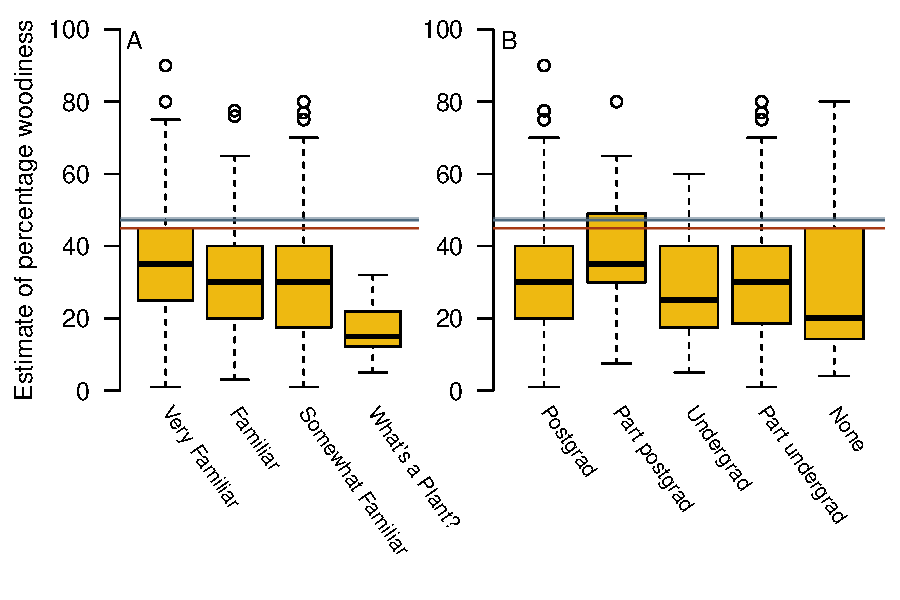
\includegraphics{figs/survey-results}
  \caption{Distribution of responses to the survey question ``What
    percentage of the world's vascular plant species are
    woody?''. Responses are divided by familiarity with plants
    (panel A) and formal training in botany or a related discipline
    (panel B). The mean and 95\% confidence intervals for our
    estimates of the proportion of woody species from the empirical
    data are depicted by the horizontal shaded rectangles; the blue
    upper rectangle corresponds to the ``weak prior'' approach and the
    red lower rectangle corresponds to the ``strong prior'' approach
    (see Appendix for details).}
  \label{fig:survey}
\end{figure}

\clearpage
\renewcommand\thefigure{S.\arabic{figure}}
\renewcommand\thetable{S.\arabic{table}}
\setcounter{figure}{0}    
\setcounter{table}{0}

\begin{figure}[p]
  \centering
  \includegraphics{figs/fraction-by-family}
  \caption{Distribution of the percentage of woodiness among families.
    The distribution of the percentage of species that are woody within
    a family is strongly bimodal among families (panel A), though less
    strongly bimodal than among genera.
    % 
    The two different sampling approaches generate distributions that
    differ in their bimodality (panel B).  Using the weak prior
    approach generates a broad distribution with many polymorphic
    genera (blue line), while using the strong prior approach
    generates a strongly bimodal distribution (red line).}
  \label{fig:distribution-family}
\end{figure}

\begin{figure}[p]
  \centering
  \includegraphics{figs/fraction-by-order}
  \caption{Distribution of the percentage of woodiness among orders.
    The distribution of the percentage of species that are woody within
    an order is bimodal among orders (panel A), though
    less strongly bimodal than among both genera and families.
    % 
    The two different sampling approaches generate distributions that
    differ in their bimodality (panel B).  Using the weak prior
    approach generates a broad distribution with many polymorphic
    genera (blue line), while using the strong prior approach
    generates a strongly bimodal distribution (red line).}
  \label{fig:distribution-order}
\end{figure}

\begin{figure}[p]
  \centering
  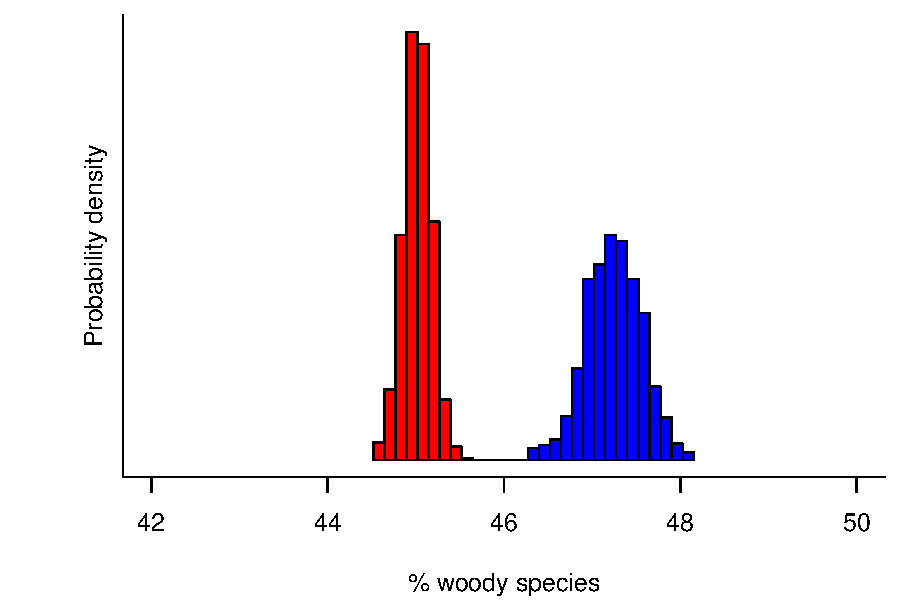
\includegraphics{figs/distribution-raw}
  \caption{(Supplementary) The posterior probability distribution for
    the proportion of the world's flora that is woody, using our two
    sampling approaches.  The red (left) distribution samples missing
    species using the strong prior approach (binomial distribution),
    while the blue distribution (right) samples missing species using
    the weak prior approach (hypergeometric distribution).}
  \label{fig:distribution-raw}
\end{figure}

\begin{figure}[p]
  \centering
  \includegraphics{figs/fraction-on-phylogeny-supp}

  \caption{(Supplementary)
    \textit{This is Fig. \ref{fig:phylogeny} using the alternative
      sampling approach.}\\
    %
    Distribution of the fraction of woodiness among orders of vascular
    plants.  Each tip represents an order, with the fraction of
    circumference proportional to the square root of the number of
    recognised species in that order (data from accepted names in
    \citet{ThePlantList}).  The bars around the perimeter indicate the
    percentage of woody (black) and herbaceous (white) species,
    estimated using the ``weak prior'' (hypergeometric) approach.
    Using the ``strong prior'' (binomial) approach generally leads to
    an estimated percentage that is further away from 50\% (see
    Figs. \ref{fig:phylogeny} and \ref{fig:distribution-genera}).
    Phylogeny from \citet{Zanne} (available on Dryad; 
    doi:10.5061/dryad.63q27/3). Orders not placed by APG III
    \citep{APG3} are not displayed.}
  \label{fig:phylogeny-supp}
\end{figure}

\begin{figure}[p]
  \centering
  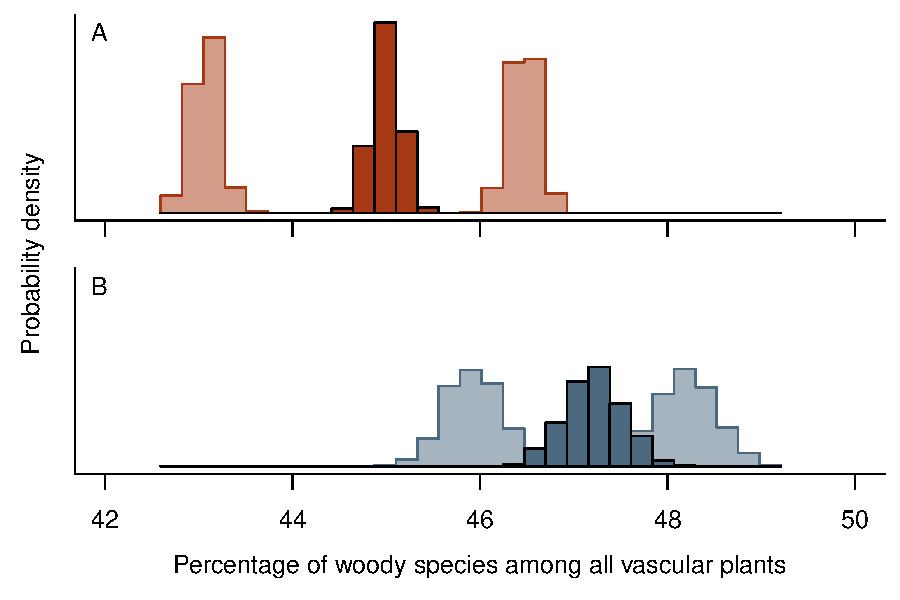
\includegraphics{figs/distribution-raw-errors}
  \caption{(Supplementary) The effect of different coding on estimates
    of the fraction of species that are woody, under the strong prior
    approach (binomial; panel A) and weak prior approach
    (hypergeometric; panel B).  The dark distributions are the results
    from our main analysis (Fig. \ref{fig:distribution-raw}).
    Distributions to the left (with lower estimates of woodiness) code
    all species with any record of herbaceousness or variability as
    herbaceous.  Similarly, distributions to the right (with higher
    estimates of woodiness) code all species with any record of
    woodiness or variability as woody.}
  \label{fig:distribution-raw-errors}
\end{figure}
    
      
\begin{figure}[p]
  \centering
  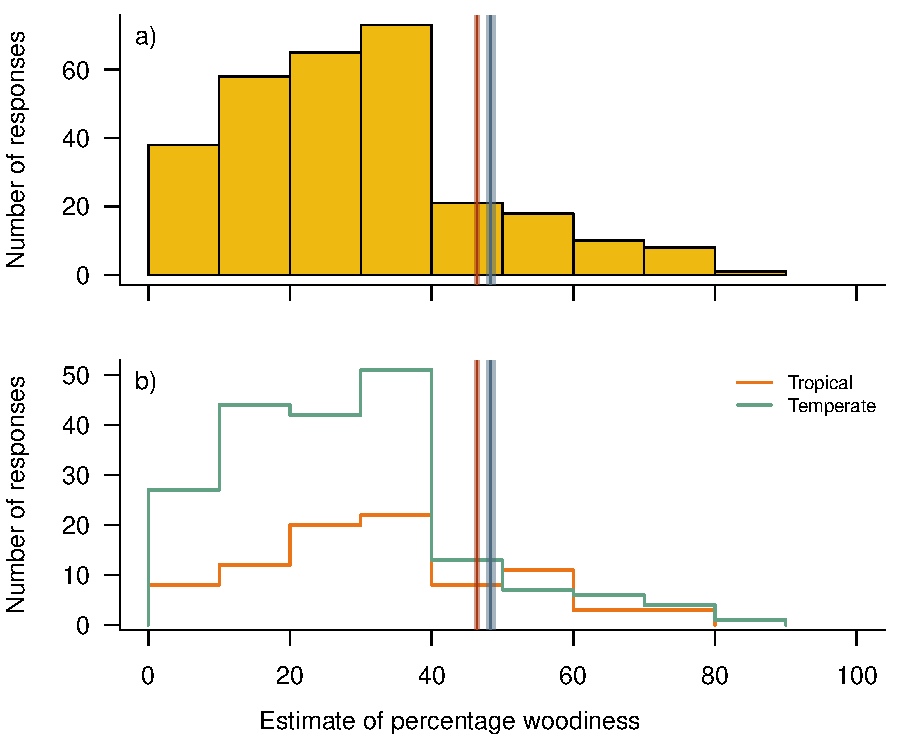
\includegraphics{figs/survey-distribution}
  \caption{(Supplementary) Distribution of all responses to the survey
    question ``What percentage of the world's vascular plant species
    are woody?''.
    %
    The mean and 95\% confidence intervals for our estimates of the
    proportion of woody species from the empirical data are depicted
    by the horizontal shaded rectangles; the blue rectangle
    corresponds to the ``weak prior'' approach and the red rectangle
    corresponds to the ``strong prior'' approach (see Appendix for
    details).  
    % 
    Panel A includes all 292 responses.  In panel B, the 282
    responses that indicated country are shown separated into
    ``tropical'' (orange distribution) and ``temperate'' (teal).
    Estimates from tropical countries were slightly, but
    significantly, higher than those from temperate countries
    ($p=$0.02, $r^2$=0.02).
    % #rstats
    % nrow(d.survey)                   # 292
    % sum(!is.na(d.survey$Country))    # 282
    % summary(res.tro)
  }

  \label{fig:survey-distribution}
\end{figure}





\begin{figure}[p]
  \centering
  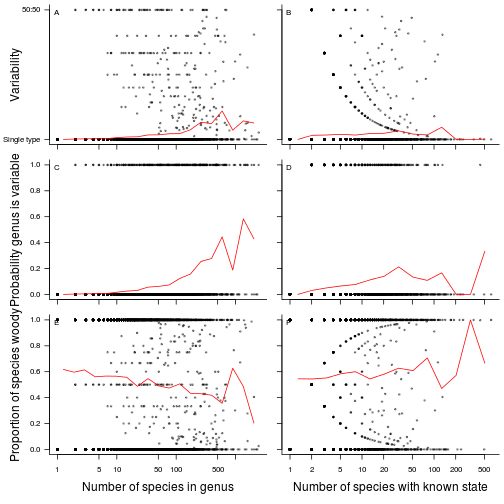
\includegraphics[scale=0.7]{figs/variability}
  \caption{(Supplementary) The relationship between the size of a genus
and its chance of being ``variable'' for woodiness.
%
We plotted the relationship between the level of variablitiy in the
dataset (from all of a single--type to equal numbers of woody and
herbaceous species) against the number of species in a genus (panel A)
and the number of species with known state (panel B). Larger genera
tend to be more variable although this pattern is not strong. We then
coded all genera as being either variable or all of a single--type and
examined the relationship between this binary characterization and the
number of species per genus (panel C) and the number for which we
have known states (panel D). Using the binary characterization, it is
clear that large genera have a higher probability of being variable,
even if few species actually vary (compare with panels A and
B). Though there is a great deal of scatter, larger genera also tend to be
more herbaceous than woody genera (panel E) but the genera for which
we have more data tend to be more woody (panel F). This shows that the
available data is generally biased towards woody species.  In all
panels, the red line is a moving average over 20 (left column) of 15 (right
column) equally spaced bins on this log axis.}
  \label{fig:variability}
\end{figure}

\begin{figure}[p]
  \centering
  \vspace{-20ex}
  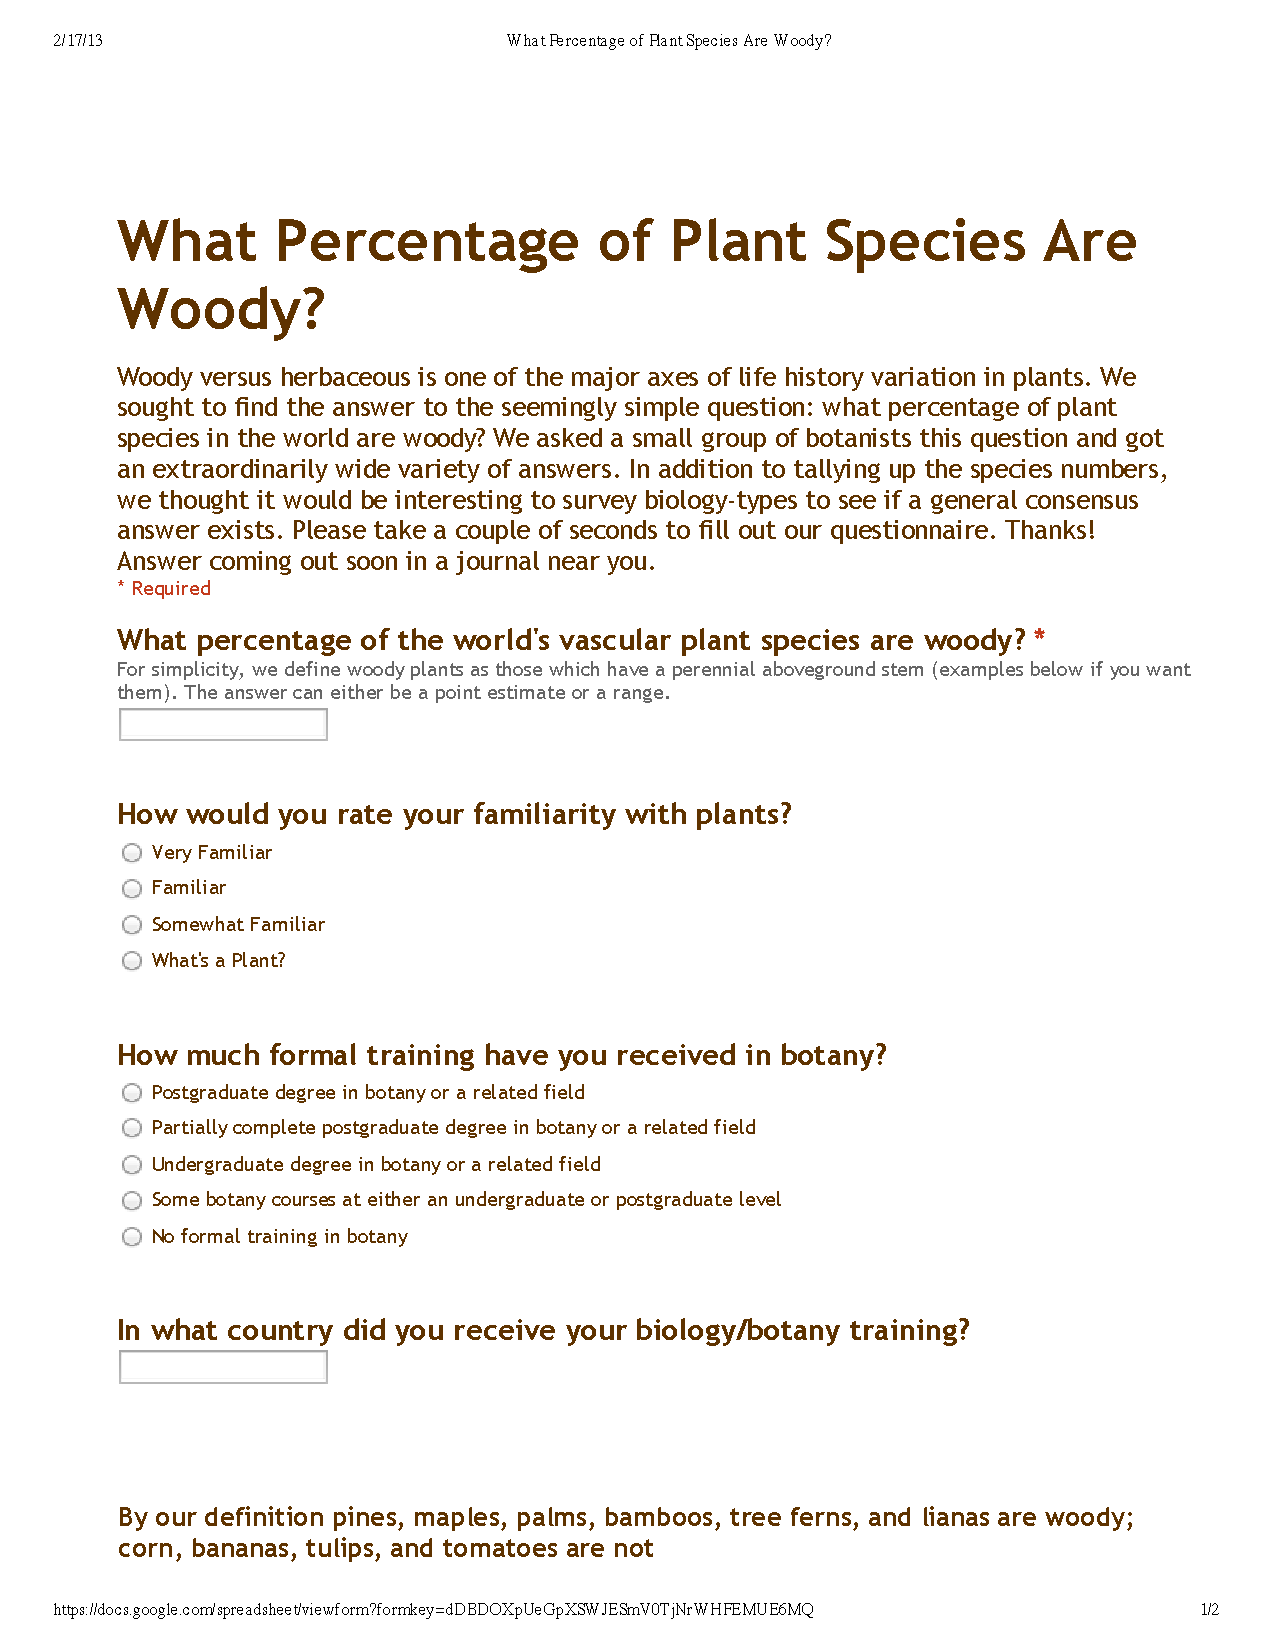
\includegraphics[scale=0.7]{figs/Survey_supplemental}
  \caption{(Supplementary) English--language version of the survey we
    distributed}
  \label{fig:survey-text}
\end{figure}

\begin{figure}[p]
  \centering
  \vspace{-20ex}
  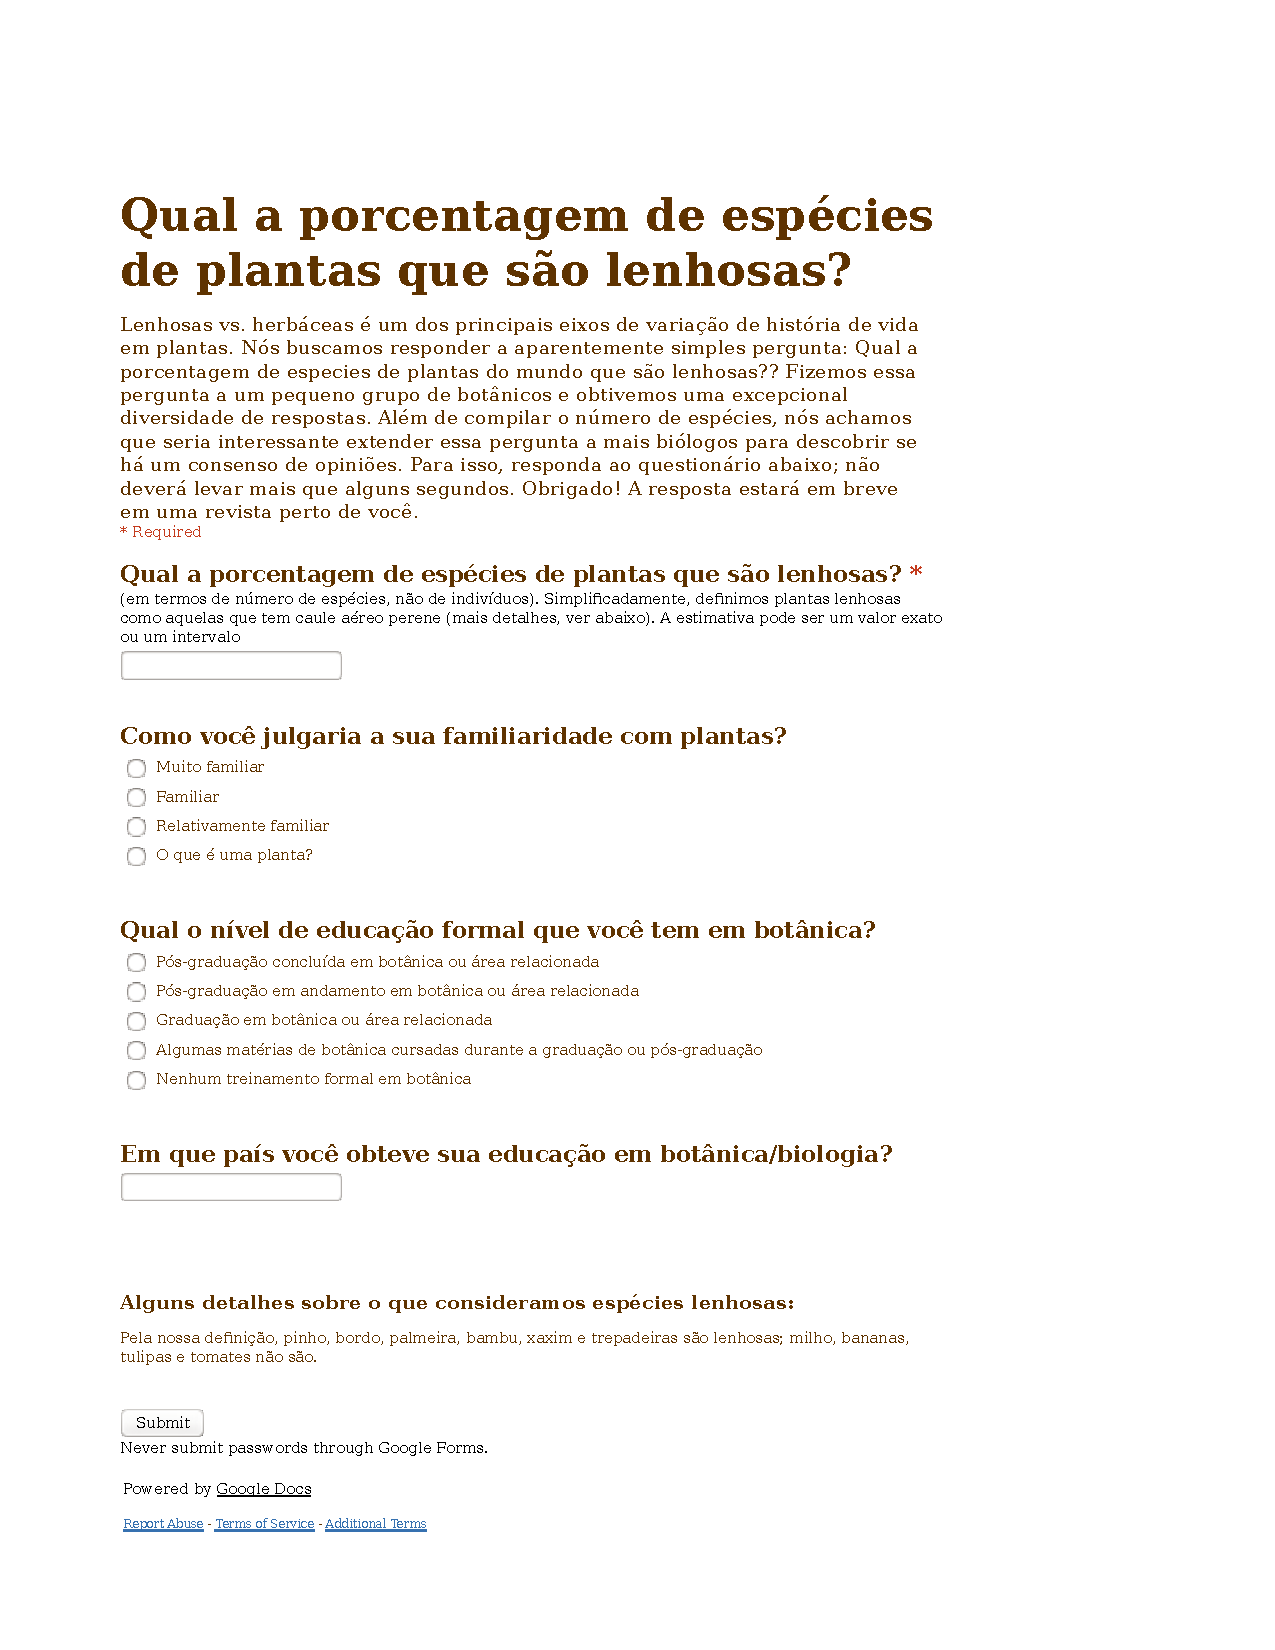
\includegraphics[scale=0.8]{figs/Survey_supplemental_Portuguese}
  \caption{(Supplementary) Portuguese--language version of the survey we
    distributed}
  \label{fig:survey-text-port}
\end{figure}

\end{document}

%%% Local Variables:
%%% mode: latex
%%% TeX-master: t
%%% TeX-PDF-mode: t
%%% End:


